\sezione{Esercizio di Dimensionamento}
Si consideri il sistema in esame formato da motore, riduttore, vite, madrevite, carico e con una legge di moto come in figura.\label{EsercizioDimRid}

\begin{figure}[h]
    \centering
    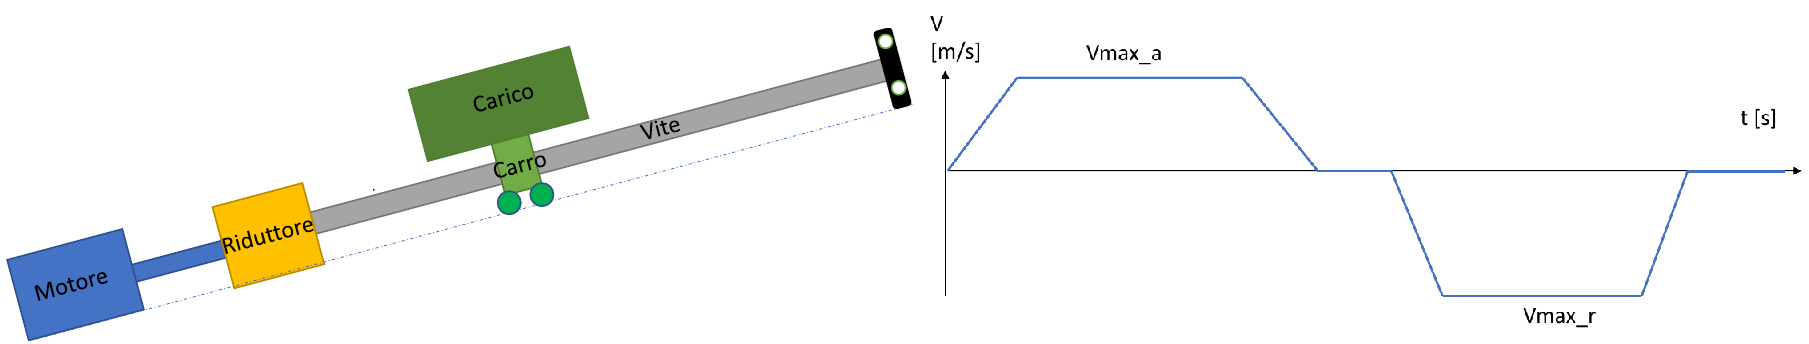
\includegraphics[width=0.8\textwidth]{Immagini/esercizio1_dim_rid_vite.png}
    \caption{Esercizio 1 dimensionamento: schema e legge oraria}
\end{figure}

\sottosezione{Step di risoluzione}
\begin{enumerate}[label=(\roman*)]
    \item Convenzioni di segno (intanto raggruppando le forze applicate su uno stesso punto)
    \item Modello (cinematico, dinamico)
    \item Manipolazione algebrica del modello per evidenziare $T_2$ ed eventualmente le forze che vanno a determinare il tipo di moto (diretto vs retrogrado)
    \item Analisi di ogni fase
    \item Valutazione del duty cycle
    \item Definizione $T_2$, scelta taglia
    \item Calcolo limitazioni alla scelta di $\tau_r$
    \item Scelta di $\tau_r$
\end{enumerate}

\paragrafo{Attrito}
Per il calcolo delle forze di attrito in regime di moto variabile è utile esplicitare le forze che vanno a determinare il tipo di moto (diretto o retrogrado) nelle espressioni della coppia di motore.
Inoltre occorre valutare con attenzione il verso secondo la convenzione utilizzata (non necessariamente coincide col significato fisico).

\sottosezione{Tabella}
Per aiutarsi nella esecuzione dei passaggi è consigliato l'utilizzo di una tabella in cui siano distinte le varie tipologie operative divise per le rispettive durate di modo da schematizzare l'esercitazione.

\begin{table}[h]
\centering
    \begin{tabular}{l|l|l|l|l|l|l|l|l|l}
    \hline
    $\Delta t$ $[s]$ & $0.4$ & $1.2$ & $0.4$ & $0.4$ & $0.3$ & $0.9$ & $0.3$ & $0.6$ & Valore massimo \\ \hline
    $\dot x$ $[m/s]$ & &  &  &  &  &  &  &  & \\ \cline{1-1}
    $\Ddot x$ $[m/s^2]$ &  &  &  &  &  &  &  &  &  \\ \cline{1-1}
    $M$ $[Kg]$ &  &  &  &  &  &  &  &  &  \\ \cline{1-1}
    \hline
    $M \Ddot x$ $[N]$ &  &  &  &  &  &  &  &  &  \\ \cline{1-1}
    $F_{p,\parallel}$ $[N]$ &  &  &  &  &  &  &  &  &  \\ \cline{1-1}
    $F_{cou}$ $[N]$ &  &  &  &  &  &  &  &  &  \\ \cline{1-1}
    $\Delta F_{cou}^s$ $[N]$ &  &  &  &  &  &  &  &  &  \\ \cline{1-1}
    \hline
    $F_{A,medi}$ $[N]$ &  &  &  &  &  &  &  &  &  \\ \cline{1-1}
    $F_{A,pk}$ $[N]$ &  &  &  &  &  &  &  &  &  \\ \cline{1-1}
    Flusso $W$ &  &  &  &  &  &  &  &  &  \\ \cline{1-1}
    \hline
    $\VelAng_v$ $[rpm]$ &  &  &  &  &  &  &  &  &  \\ \cline{1-1}
    $\AccAng_v$ $[rd/s]$ &  &  &  &  &  &  &  &  &  \\ \cline{1-1}
    \hline
    $J_v\AccAng_v$ $[Nm]$  &  &  &  &  &  &  &  &  &  \\ \cline{1-1}
    $T_2$ $[Nm]$ &  &  &  &  &  &  &  &  &  \\ \cline{1-1}
    $T_{2,pk}$ $[Nm]$ &  &  &  &  &  &  &  &  &  \\ \cline{1-1}
    \end{tabular}
    \caption{Tabella riassuntiva per i calcoli effettuati}
\end{table}

\paragrafo{Incremento di Attrito:}
Con $\Delta F_{Cou}$ si intende l'incremento di attrito legato alla differenza tra attrito statico e dinamico; nota bene che $\Delta F_{Cou} + F_{Cou} \leqslant F_{motrice}$, quindi l'incremento potrà al massimo far sì che l'oggetto rimanga fermo, non può mettere in moto.

\paragrafo{Attrito di Primo Distacco:}
L'attrito statico è di primo distacco interviene quando si passa da arresto a moto, tuttavia il tempo di applicazione dell'attrito è ridotto rispetto il ciclo di lavoro, perciò può influenzare il valore di picco di forza\footnote{Questo non andrà a influenzare la scelta del motore perché i motori brushless tendono ad avere coppie di spunto alte a sufficienza per garantire il primo distacco.}, ma non la media. Questi casi vengono segnati in tabella mettendo il valore entro parentesi tonde.

\paragrafo{Verifica segni:}
Per verificare di aver utilizzato tutte le convezioni corrette conviene partire dai segni dell'inerzia, valutare in base alla legge oraria quale sia il segno dell'inerzia resistente e quale dell'inerzia motrice, e infine estendere quanto ricavato alle altre forze, quindi verificare che le forze resistenti e motrici siano concordi coi segni delle rispettive inerzie.
Nell'esempio occorrerà valutare il segno dell'inerzia resistente e motrice nelle condizioni di salita e discesa.

\paragrafo{Rivalutazione coefficiente di sicurezza:}
Facendo l'esercizio ci si accorge che utilizzando un coefficiente di sicurezza del $20\%$ non si trova un riduttore tra quelli a disposizione perché la velocità media richiesta è troppo elevata. L'unica opzione\footnote{Vedi quanto detto a pagina \pageref{rivalutazione_coeff_sic}} è modificare il coefficiente di sicurezza.
In questo caso particolare la $T_{2,media}$ è circa la metà di quella nominale, perciò termicamente il rischio è minimo, quindi è possibile abbassare il coefficiente di sicurezza relativo alla velocità media.